\documentclass[sigconf]{acmart}

\usepackage{algorithmic}
\usepackage{algorithm}
\usepackage{hyperref}
\usepackage[newfloat,cache=false]{minted}

\begin{document}

\title{COMP6247 - Recursive Least Squares}
\author{Luke McClure}
\email{29573904}

\maketitle
\pagestyle{myheadings} 

%% Pull all includes into here so no page breaks
\section{Linear regression by several forms}
\subsection{Closed Form}

\begin{listing}[H]
    \begin{minted}[frame=lines, breaklines, breaksymbolleft=, fontsize=\footnotesize]{python}
def linReg(X, y):
    weights = np.linalg.inv(X.T @ X) @ X.T @ y
    preds = X @ weights
    return preds, weights
    \end{minted}
\end{listing}

\subsection{Gradient Descent}

\begin{listing}[H]
    \begin{minted}[frame=lines, breaklines, breaksymbolleft=, fontsize=\footnotesize]{python}
def linRegGD(X, y, iters, l=0.00001):
    weights = np.zeros((features, 1))
    
    iterations = np.empty(iters)
    for i in range(iters):
        update = 2 * X.T @ ((X @ weights) - y)
        weights = weights - l * update
        iterations[i] = np.linalg.norm(y - X @ weights)
    
    preds = X @ weights
    return preds, weights, iterations
    \end{minted}
\end{listing}

\subsection{Stochastic Gradient Descent}

\begin{listing}[H]
    \begin{minted}[frame=lines, breaklines, breaksymbolleft=, fontsize=\footnotesize]{python}
def linRegSGD(X, y, iters, l=0.05):
    weights = np.zeros((X.shape[1], 1))
    iterations = np.empty(iters)
    
    for i in range(iters):  
        j = np.floor(np.random.rand()*X.shape[0]).astype(int)
        error = (X[j] @ weights) - y[j]
        update = error * X[j].T
        weights = weights - l * update.reshape(update.shape[0], 1)
      
        iterations[i] = np.linalg.norm(X @ weights - y)
        
    preds = X @ weights
    return preds, weights, iterations
    \end{minted}
\end{listing}

\subsection{Comparisons}
\begin{center}
    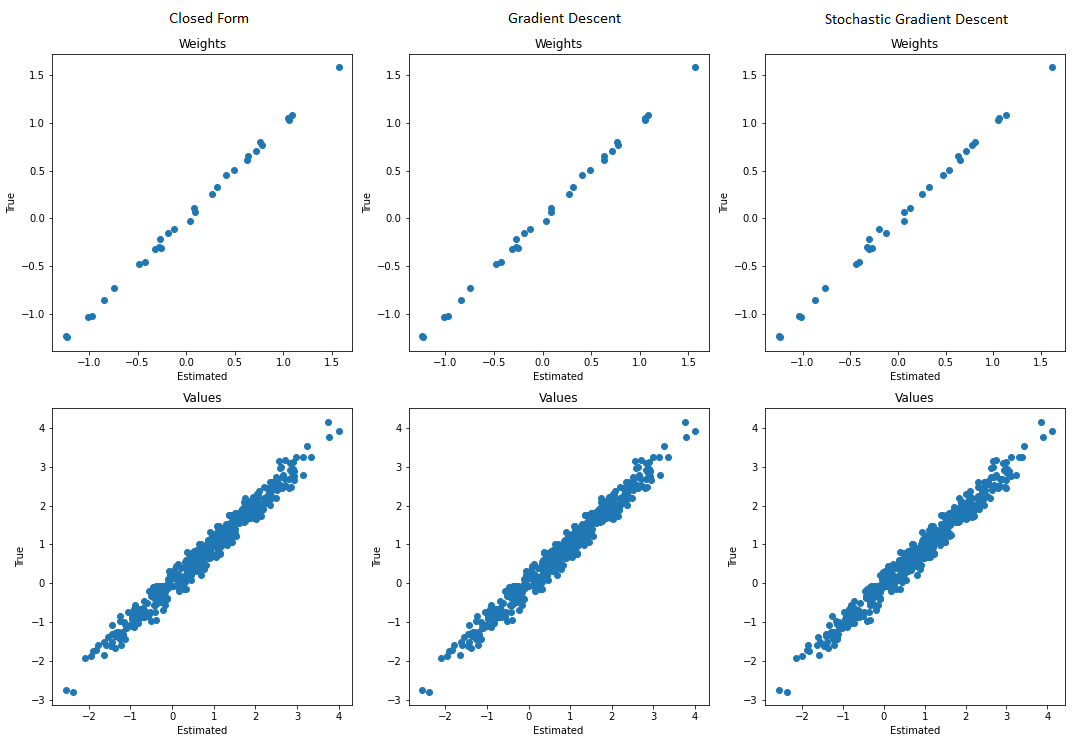
\includegraphics[width=\linewidth]{figs/LinRegComparison.png}
\end{center}

To put a numerical figure on the accuracy of learning between these methods, I compared the true weights of the data to the weights that were found by each method using MSE. 
\begin{center}
    \begin{tabular}{| c c |}
        \hline
        Algorithm & Weight MSE \\ 
        \hline\hline
        Closed Form & $7.298 \times 10^{-4}$\\ 
        Gradient Descent & $7.294 \times 10^{-4}$ \\
        Stochastic Gradient Descent & $1.900 \times 10^{-3}$\\
        \hline      
    \end{tabular}
\end{center}
With careful tuning, the weights MSE between closed form and gradient descent were brought to within 0.05\% of each other. 
This shows how the closed form method and gradient descent are the most accurate at replicating the true weights, although this requires delicate tuning to get the performance in GD. Stochastic Gradient Descent follows these methods by a factor of 10.

Gradient Descent over the whole dataset provides a very smooth error graph. By effectively averaging the update that needs to be done for every data point and using this to update the weights provides a much smoother descent to the minimum.
Stochastic Gradient Descent on the other hand is noisy, the loss has iterations where it will increase instead of decrease which means it can be uncertain when to stop. This is due to the single sample nature of this algorithm, by updating the weights using only a single sample the change will not capture the entire dataset and result in the algorithm jumping around a local minima while not settling in it.

\begin{center}
    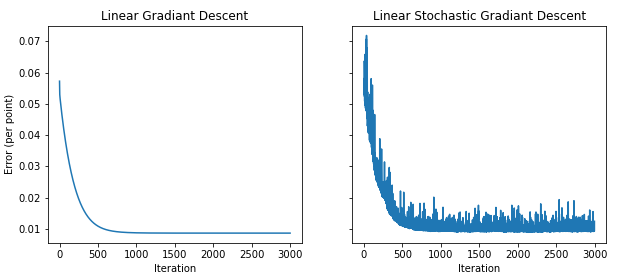
\includegraphics[width=\linewidth]{figs/GD vs SGD.png}
\end{center}

As a result of the fuzzy nature of Stochastic Gradient Descent the final error of the algorithm is not quite as low as Gradient Descent. 
\subsection{Improving SGD}
To combat the issue of jumping loss within SGD I implemented a technique where the learning rate is lowered proportionally to the iteration through the dataset. By gradually lowering the learning rate in this fashion the steps the algorithm takes when updating the weights gets lower and lower, eventually converging on to the local minima instead of jumping around a value.
\begin{listing}[H]
    \begin{minted}[frame=lines, breaklines, breaksymbolleft=, fontsize=\footnotesize]{python}
def linRegSGD_smoothed(X, y, iters, lb=0.05, le=None):
    if(le==None):
        le = lb/10
    weights = np.zeros((X.shape[1], 1))
    #decrease learning rate through iterations
    l = np.linspace(lb,le,iters)
    iterations = np.empty(iters)
    
    for i in range(iters):  
        j = np.floor(np.random.rand()*X.shape[0]).astype(int)
        update = ((X[j] @ weights) - y[j]) * X[j].T
        weights = weights - l[i] * update.reshape(update.shape[0], 1)
      
        iterations[i] = np.linalg.norm(X @ weights - y)
        
    preds = X @ weights
    return preds, weights, iterations
    \end{minted}
\end{listing}
This succeeds in smoothing the error across iterations within SGD, but at the detriment of further increasing the error score of this algorithm at the end of iterations.

\begin{center}
    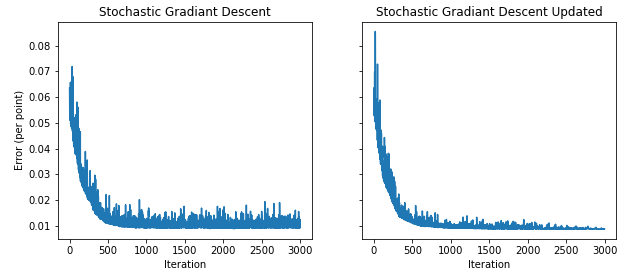
\includegraphics[width=\linewidth]{figs/SGDFixed.png}
\end{center}

\section{Recursive Least Squares}
\subsection{Implementation}
\begin{listing}[H]
    \begin{minted}[frame=lines, breaklines, breaksymbolleft=, fontsize=\footnotesize]{python}
def RLS(X, y, lam, eps=0.01):
    #initialisations
    weights = np.zeros((X.shape[1], 1))
    P = (1/eps)*np.identity((X.shape[1]))
    lami = lam**(-1)

    #vis initialisations
    iterError = np.empty(X.shape[0])
    errorAll = np.empty((X.shape[0]))
    randError = np.empty((X.shape[0]))
    

    for i in range(X.shape[0]):
       #algorithm
        xn = X[i].reshape(-1, 1)
        pred = weights.T @ xn 
        error = y[i] - pred
        k = (lami * P @ xn) / (1 + lami * xn.T @ P @ xn)
        P = (lami * P) - (lami * k @ xn.T @ P)  
        weights += (k * error)
        
        #visualisation
        iterError[i] = np.linalg.norm(error)
        errorAll[i] = np.linalg.norm(y - X @ weights)
        j = np.floor(np.random.rand()*X.shape[0]).astype(int)
        predRand[i] = np.linalg.norm(y[j] - weights.T @ X[j])
        
    return weights, iterError, errorAll, randError
    \end{minted}
\end{listing}

\subsection{Performance}
Recursive Least Squares is able to match the numerical performance of the Closed Form and Gradient Descent methods very well.

\begin{center}
    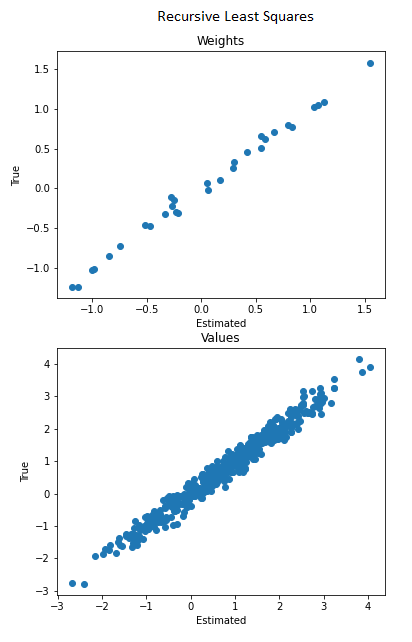
\includegraphics[scale= 0.4]{figs/RLS Weights.png}
\end{center}

By performing the same comparison of the learnt weights to their true values, it is shown that RLS is within a factor of 10 of Stochastic Gradient Descent.
\begin{center}
    \begin{tabular}{| c c |}
        \hline
        Algorithm & Weight MSE \\ 
        \hline\hline
        Closed Form & $7.298 \times 10^{-4}$\\ 
        Gradient Descent & $7.294 \times 10^{-4}$ \\
        Stochastic Gradient Descent & $1.900 \times 10^{-3}$\\
        Recursive Least Squares & $5.890 \times 10^{-3}$\\
        \hline      
    \end{tabular}
\end{center}
Recursive Least Squares manages to fit to the data very quickly, within the first 50 values seen by the model the error per point is below 0.5.

\begin{center}
    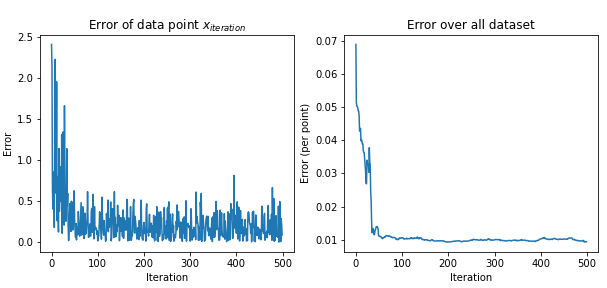
\includegraphics[width=\linewidth]{figs/RLS Error of points.png}
\end{center}
By building up a model of the covariance within the data point by point, this learning scales very quickly to the entire dataset. Within 50 iterations the error over the entire dataset is around 0.01 per point, compared to iteration 500 with GD and SGD.
\subsection{Convergence vs Dimensionality}
To investigate how quickly RLS is able to converge dependant on the dimensionality of the sample data, first we must decide when the algorithm has appropriately converged.

I decided that I would set a threshold for the boundary using the mean and standard deviation of the error, and once a bounds percentage of the data was below this threshold that would be set as the iteration of convergence.
As the error per data point seen on every iteration has a wider variance, the threshold was set at mean + 1 standard deviation. Once 95\% of the future error was under this threshold that iteration was decided as the iteration for convergence.
Error over the entire dataset has a much smoother curve, the threshold was set at the mean of the error and the bounds percentage was set to 100\% due to this smoothness. 
The plots for these are shown with the threshold shown using a horizontal red line, and the iteration of convergence shown using a vertical green line. 

\begin{center}
    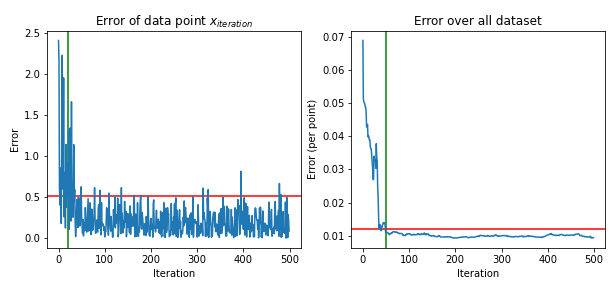
\includegraphics[width=\linewidth]{figs/RLS Error W Lines.png}
\end{center}

Using the error over the entire dataset yielded a much more stable prediction of the iteration of convergence.

For a number of samples sizes ranging from 5 to 2 $\times$ number of features, 50 data sets are created and fitted using the RLS algorithm, the iteration of convergence is then found for each data set and the mean over is plotted in the graph below.

\begin{center}
    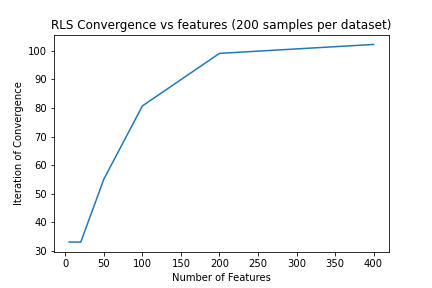
\includegraphics[width=\linewidth]{figs/RLSConvergence.png}
\end{center}
This shows clearly that as the number of features increases, so does the number of iterations needed to converge on the data.

A drawback with the method used to determine convergence is evident in these results however. By setting the iteration of convergence to the iteration where all of the future errors are below the mean, this results in the iteration of convergence being set as half the size of the dataset if it were not to converge. 
This behaviour of not converging happens as there are larger numbers of samples compared to the number of samples exposed to the model.  

\section{Comparing Stochastic Gradient Descent and Recursive Least Squares}

I used the UCI Machine Learning Repository Parkinson's Data Set\footnote{https://archive.ics.uci.edu/ml/datasets/parkinsons} for this analysis.

Using this dataset I will be attempting to predict the UPDRS, a score to rate the severity of symptoms displayed by a subject with Parkinson's. The only data the model will have available are a number of measures of measures of vocal ability displayed by the subject. These measures include maximum, average and mean vocal fundamental frequency, variation in frequency and in amplitude.

There are several features that we are not interested within this dataset, and these must be dropped to avoid the model having any extra features to attempt prediction from. The features that have been dropped include age, sex, test\_time and motor\_UPDRS.
\subsection{Single Subject}
There are 42 subjects features within the dataset, subject 12 was randomly selected to investigate the performance on a single series.

The UPDRS shows a regular cyclic pattern over the span of the measurements. There are only 107 measurements available for this subject, so it will be interesting how RLS compares to SGD as there will only be that many iterations of the algorithm compared to 3000.
\begin{center}
    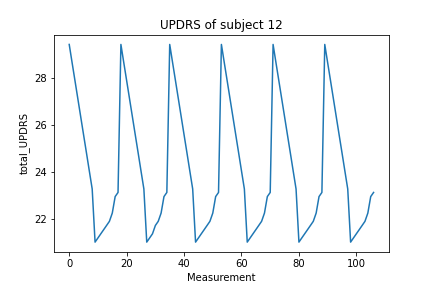
\includegraphics[width=\linewidth]{figs/Parks true single.png}
\end{center}
LinRegSGD\_smoothed was used in order to gently level the error into a single final measurement, rather than allowing for a fluctuating error, learning rate was set to 0.0005 over 300 iterations.
Stochastic Gradient Descent quickly falls to some of it's lowest errors within the first 20 iterations, this rises slowly over iterations 200-2000 before falling slowly back down to a final error per point of 0.312.

\begin{center}
    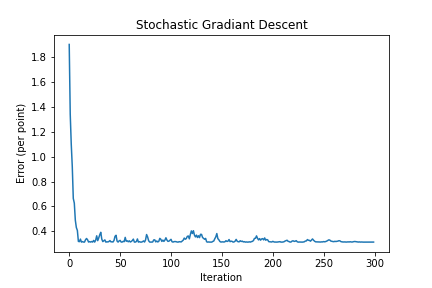
\includegraphics[width=\linewidth]{figs/Parks SGD single.png}
\end{center}

Recursive Least Squares quickly reduces the error over the entire dataset within the first 10 samples given to the model. This error per point has a slight bump before completely converging of it's final score that may be due to the model learning the cyclic pattern in the data.

Interestingly on the plot of error on the data point given the the algorithm at that point, the cyclic pattern of the data can be seen. This may be due to the algorithm initially struggling to capture these cycles and being "surprised" by them.
The final error per point from the RLS algorithm with forgetting factor 0.98 is 0.233.

\begin{center}
    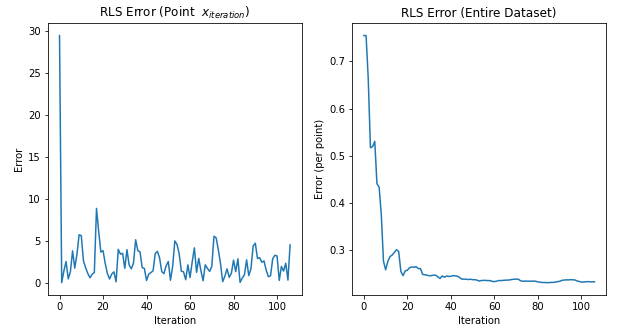
\includegraphics[width=\linewidth]{figs/Parks RLS single.png}
\end{center}
\subsection{All Subjects}
By predicting on all of these subjects independently we can get a much better picture on how these two methods are able to work with this data.
All runs over this dataset use the same parameters as with the single subject analysis.

All of the RLS runs are very similar in nature, with all of them converging to near their final error value within the first 20 iterations. Within these first twenty iterations there appears to be a block of dataset that do not converge to as low an error and the majority which very quickly converge to a similar error. Once the model has converged the error has a very low variance within a single subject.

Within the SGD runs there is one extreme outlier which does not converge until close to 50 iterations. Ignoring this data set all of the other subjects form a tighter grouping, but with more variance inside the single subjects compared to RLS. 

\begin{center}
    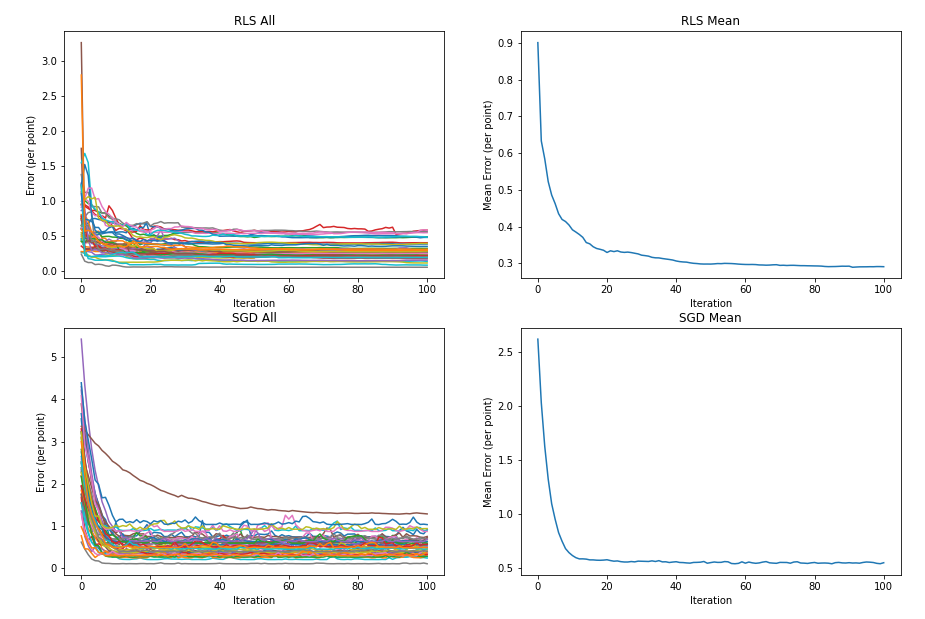
\includegraphics[width=\linewidth]{figs/ParkinsonsALL.png}
\end{center}

To provide easier analysis, all the subject datasets were combined into a single mean for each algorithm. 
The error for SGD falls sharper than RLS, but produces a much less smooth line after this initial convergence. 

The final median error per point for RLS was 0.291 whilst for SGD it was 0.550, RLS was able to converge as fast as SGD while also producing a better error score across the entire set of subjects.

\section{Comparing RLS implementations}
To compare between both implementations, I will be using the same dataset for all runs. The forgetting rate will be set to 0.98, and the P initialisation value $\epsilon$ will be set to 0.1.
The setup for this experimentation will the same as in Tasks 1 \& 2 to take advantage of the prior knowledge of true weights for the dataset.
\subsection{Original Padasip Implementation}
Padasip provides values that have a much wider variance than my implementation, these error  values are also much higher than the error values produced by my own implementation.

\begin{center}
    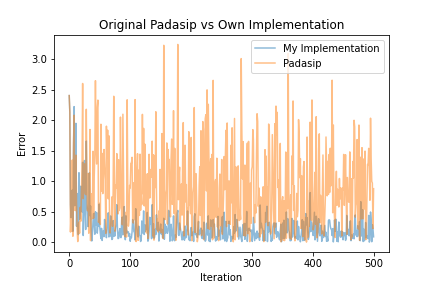
\includegraphics[width=\linewidth]{figs/OrigPadasip.png}
\end{center}

Comparing the found weights MSE compared to their true values, this difference in accuracy is apparent.
\begin{center}
    \begin{tabular}{| c c |}
        \hline
        Algorithm & Weight MSE \\ 
        \hline\hline
        Original Padasip & $4.20 \times 10^{-1}$\\ 
        My implementation & $4.71 \times 10^{-3}$\\
        \hline      
    \end{tabular}
\end{center}

\subsection{Modified Padasip Implementation}
It was noted that the Padasip implementation has a bug in it due to the shaping of data, fixing the bug using the provided code provides the following implementation.

When the bug was corrected, the Padasip implementation provided an almost exact result to my implementation.

\begin{center}
    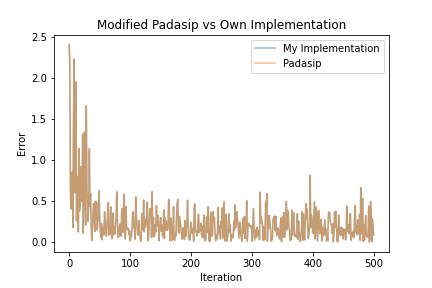
\includegraphics[width=\linewidth]{figs/ModPadasip.png}
\end{center}

The implementations are so close to one another that the MSE between the predictions performed by the two implementations is $2.81 \times 10^{-27}$ compared to 0.91 between my implementation and the original Padasip implementation. 
\end{document}
\endinput